% You should title the file with a .tex extension (hw1.tex, for example)
\documentclass[12pt]{article}\sloppy

\usepackage{amsmath}
\usepackage{amssymb}
\usepackage{fancyhdr}
\usepackage{graphicx}
\usepackage{float}
\usepackage{longtable}

\floatplacement{figure}{H}
\oddsidemargin0cm
\topmargin-2cm     %I recommend adding these three lines to increase the 
\textwidth16.5cm   %amount of usable space on the page (and save trees)
\textheight23.5cm  

\newcommand{\myname}{Abhinav Maurya}
\newcommand{\myandrew}{amaurya@andrew.cmu.edu}
\newcommand{\myhwnum}{2}

\newcommand{\question}[2] {\vspace{.25in} \hrule\vspace{0.5em} \noindent{\bf #1: #2} \vspace{0.5em} \hrule \vspace{.10in}}
\renewcommand{\part}[1] {\vspace{.10in} {\bf (#1)}}

\setlength{\parindent}{0pt}
\setlength{\parskip}{5pt plus 1pt}
 
\pagestyle{fancyplain}
\lhead{\fancyplain{}{\textbf{HW\myhwnum}}}      % Note the different brackets!
\rhead{\fancyplain{}{\myname\\ \myandrew}}
\chead{\fancyplain{}{16-720}}

\begin{document}

\medskip                        % Skip a "medium" amount of space
                                % (latex determines what medium is)
                                % Also try: \bigskip, \littleskip

\thispagestyle{plain}
\begin{center}                  % Center the following lines
{\Large 16-720: Assignment \myhwnum} \\
\myname \\
\myandrew \\
\end{center}

\question{1.1}{createGaussianPyramid}

Already provided to us in \texttt{code/createGaussianPyramid.m} file.

\question{1.2}{createDoGPyramid}

Included in \texttt{code/createDoGPyramid.m} file.

\question{1.3}{computePrincipalCurvature}

Included in \texttt{code/computePrincipalCurvature.m} file.

\question{1.4}{getLocalExtrema}

Included in \texttt{code/getLocalExtrema.m} file.

\question{1.5}{DoGdetector}

Included in \texttt{code/DoGdetector.m} file. Results in figure (\ref{fig:dogdetector}).

\begin{figure*}[f]
\centering
\begin{tabular}{| c | c |}
  \hline
  Chicken Broth Image & Duquesne Incline Image \\
  \hline
  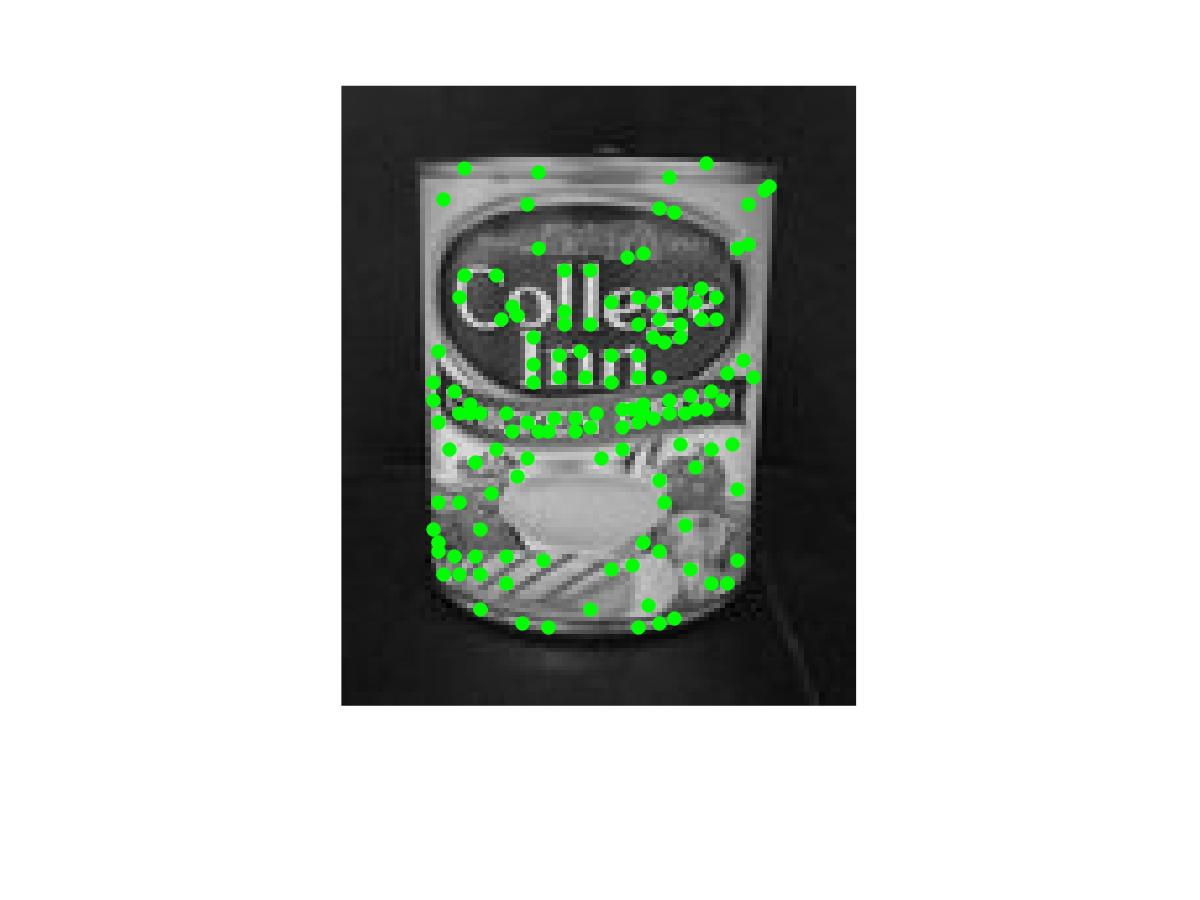
\includegraphics[trim=30mm 30mm 30mm 30mm, clip=true, width=0.45\linewidth]{../results/InterestPointsBrothGrayScale.jpg} & 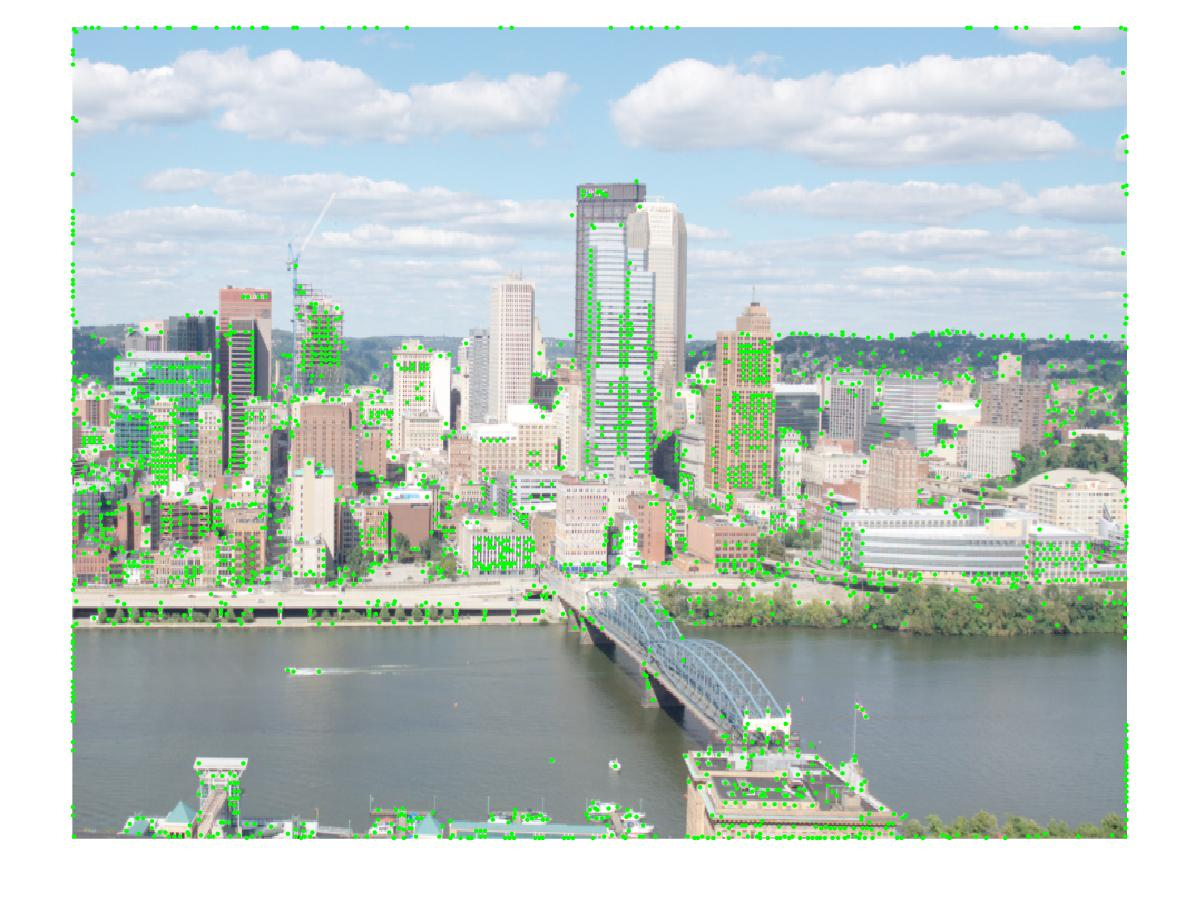
\includegraphics[width=0.45\linewidth]{../results/InterestPointsIncline.jpg} \\
  \hline
\end{tabular}
\caption{Output of \texttt{DoGDetector}}
\label{fig:dogdetector}
\end{figure*}

\question{2.1}{makeTestPattern}

Included in \texttt{code/makeTestPattern.m} file. Created pattern saved in file \texttt{code/testPattern.mat}.

\question{2.2}{computeBrief}

Included in \texttt{code/computeBrief.m} file.

\question{2.3}{briefLite}

Included in \texttt{code/briefLite.m} file.

\question{2.4}{plotMatches}

Included in \texttt{code/plotMatches.m} file. Results in figure (\ref{fig:testmatches}). We observe that rotation of the image greatly reduces the number of matches, which is observed in the matches of the original grayscale image with both the image showing all 3 textbooks in a rotated fashion as well as the three textbooks piled up and the PF textbook rotated and on top. We see a significant number of matches on the incline images where there is perspective rotation but no rotation in the plane of the image. Placing the book on the desk or against the stand leads to some reduction in the number of matches with the original grayscale textbook image. However, it is much lesser than the reduction in matches caused due to image rotation.

\begin{figure*}[f]
\centering
\begin{tabular}{| c | c |}
  \hline
  Incline Image Matches & PF Scaled and Desk Matches \\
  \hline
  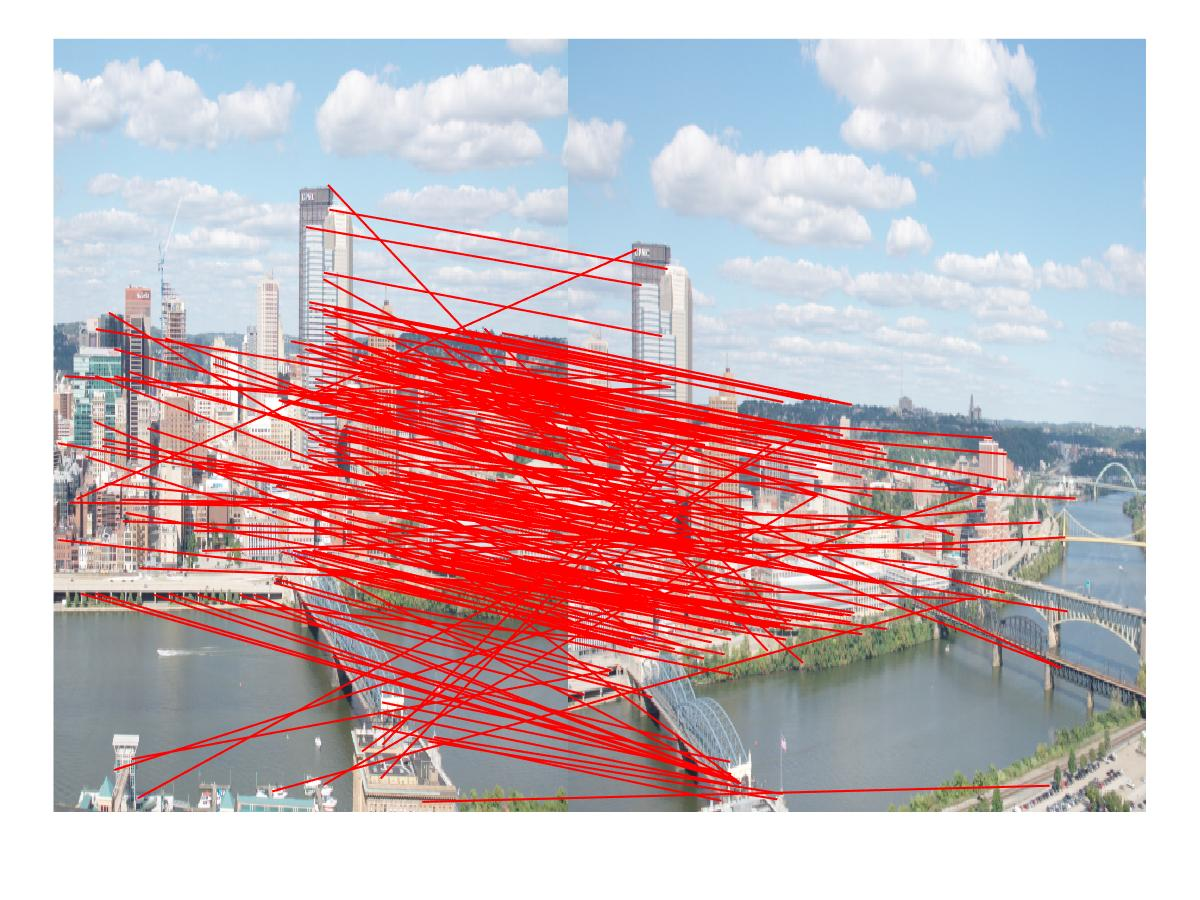
\includegraphics[width=0.42\linewidth]{../results/ImageMatchIncline.jpg} & 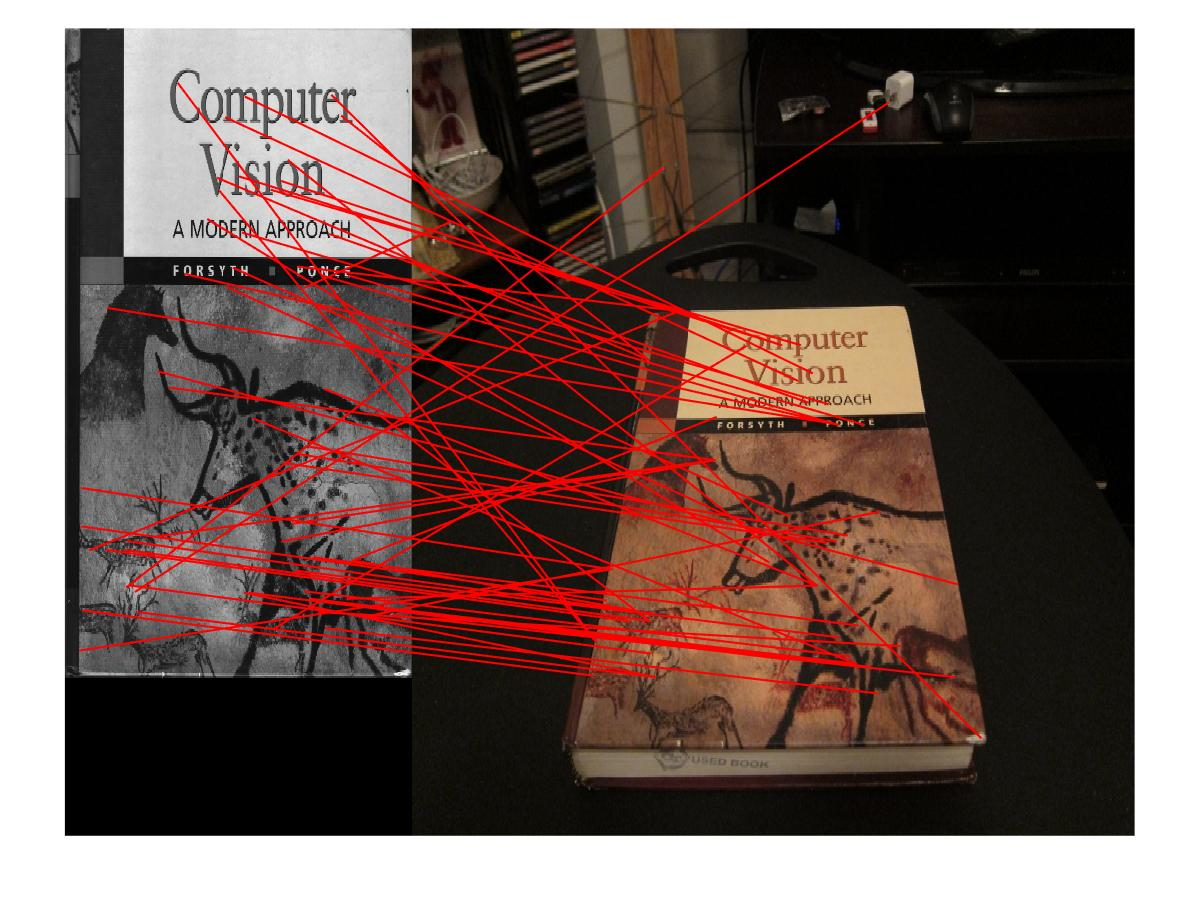
\includegraphics[width=0.42\linewidth]{../results/ImageMatchPFDesk.jpg} \\
  \hline
  PF Scaled and Floor Matches & PF Scaled and Floor Rotated Matches \\
  \hline
  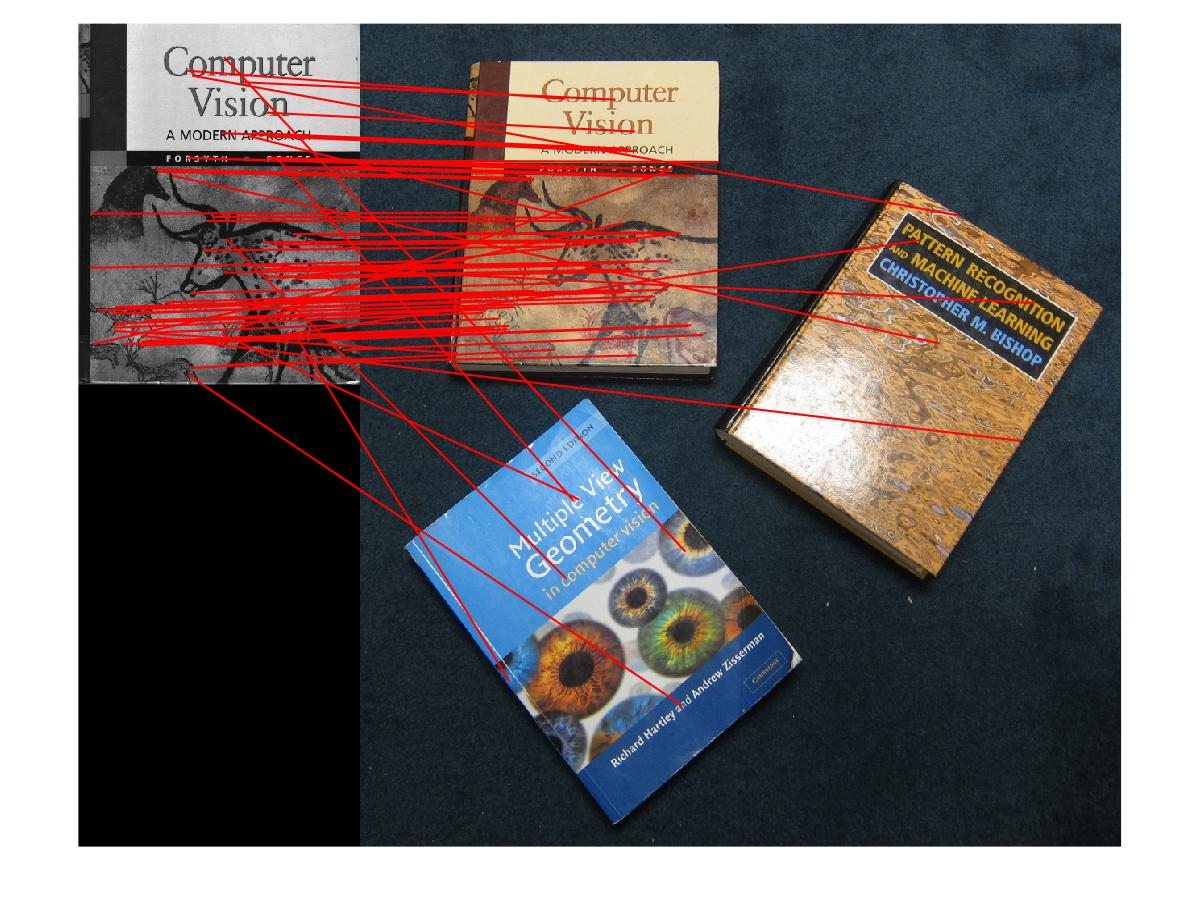
\includegraphics[width=0.42\linewidth]{../results/ImageMatchPFFloor.jpg} & 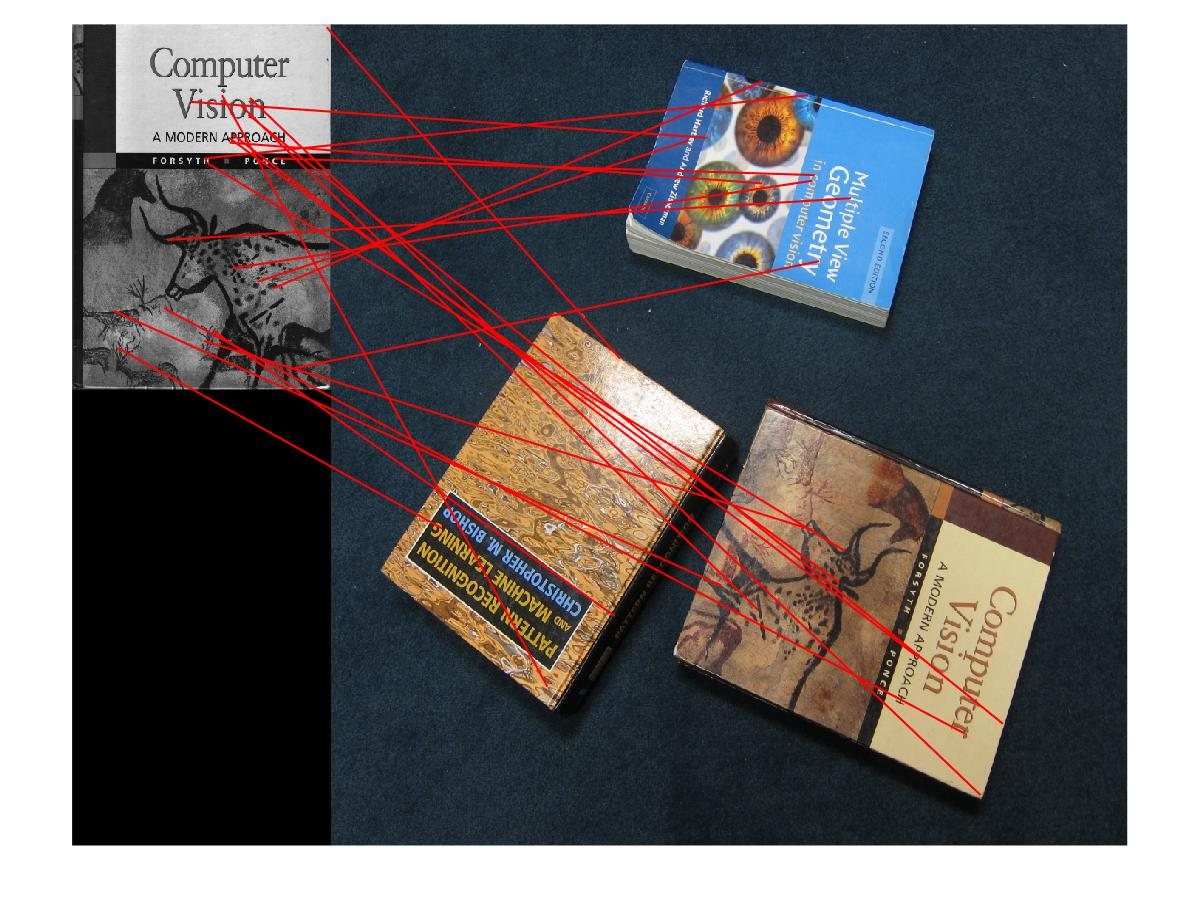
\includegraphics[width=0.42\linewidth]{../results/ImageMatchPFFloorRotate.jpg} \\
  \hline
  PF Scaled and Pile Matches & PF Scaled and Stand Matches \\
  \hline
  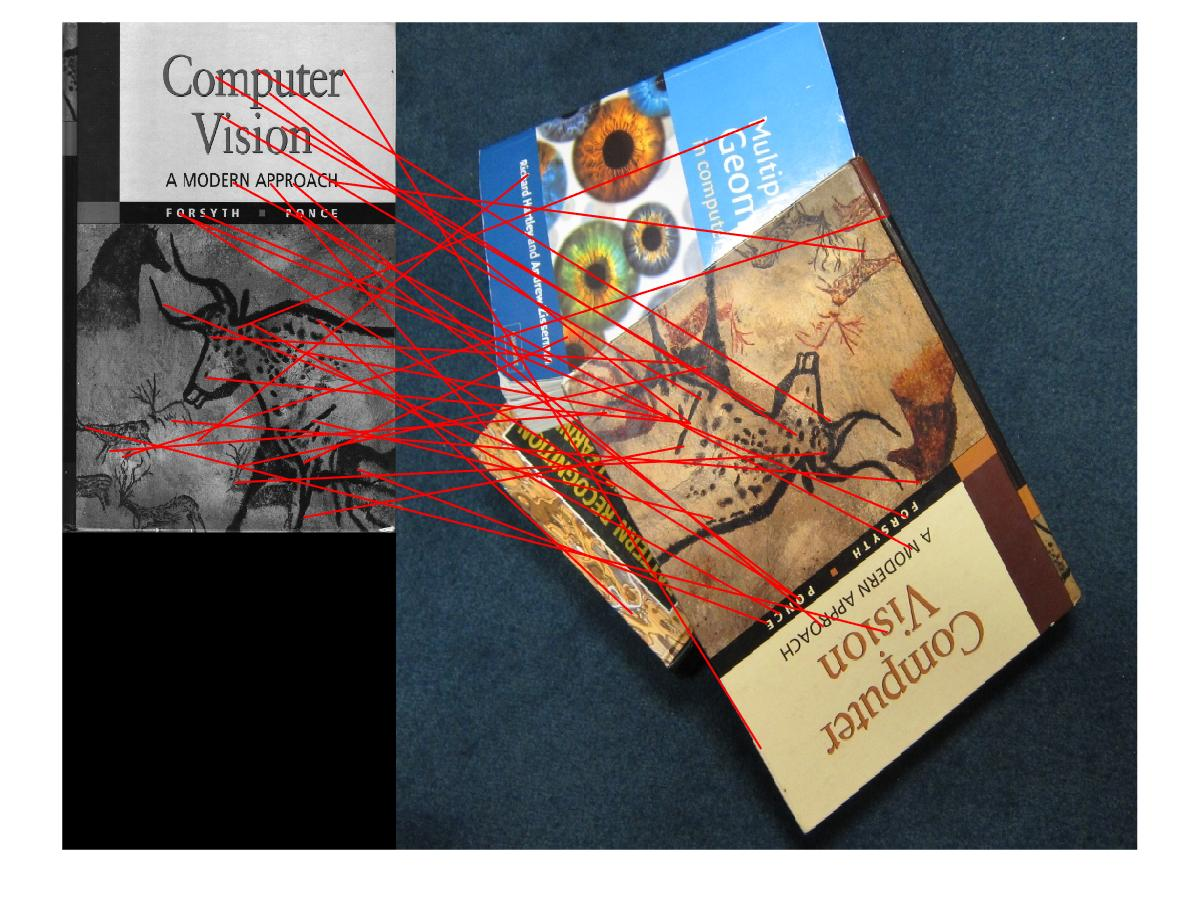
\includegraphics[width=0.42\linewidth]{../results/ImageMatchPFPile.jpg} & 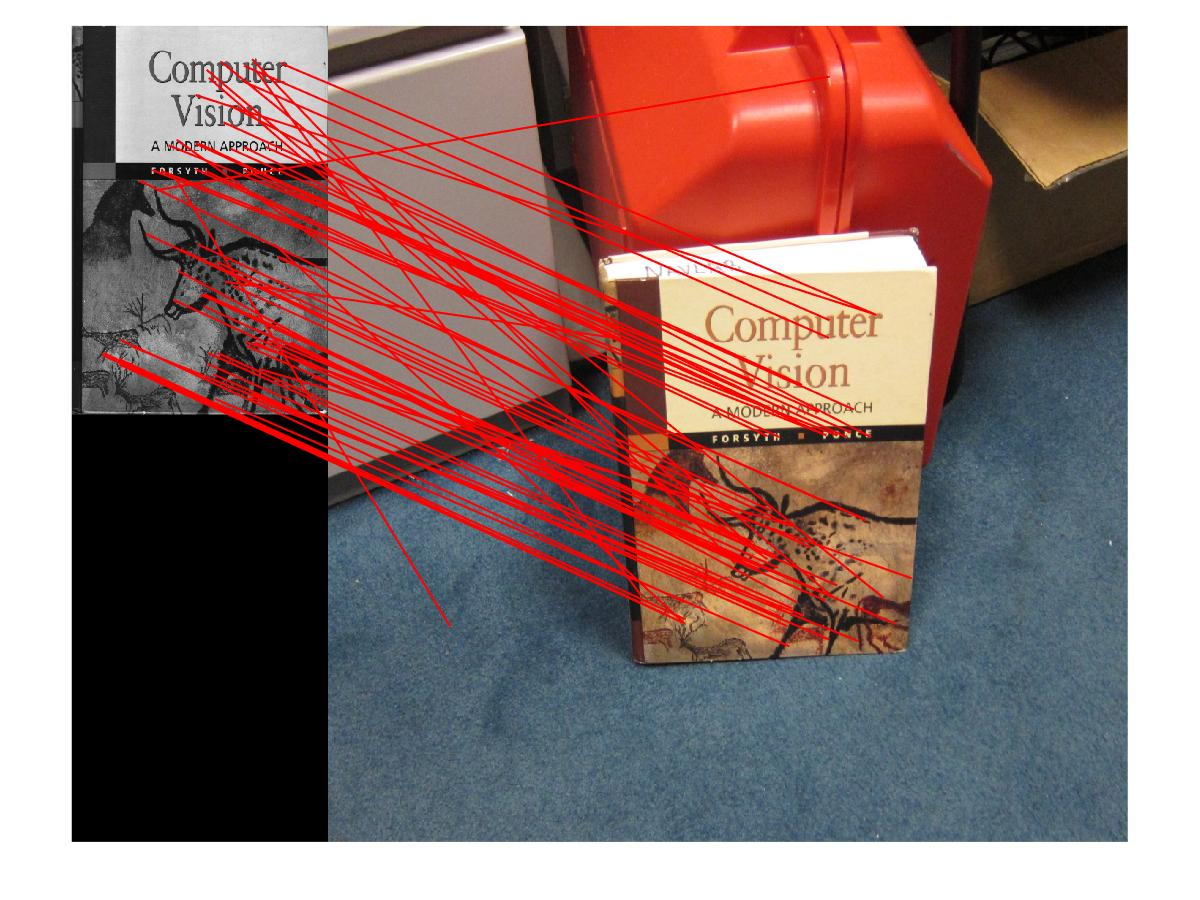
\includegraphics[width=0.42\linewidth]{../results/ImageMatchPFStand.jpg} \\
  \hline
  PF Floor and Floor Rotated Matches & PF Desk and Pile Matches \\
  \hline
  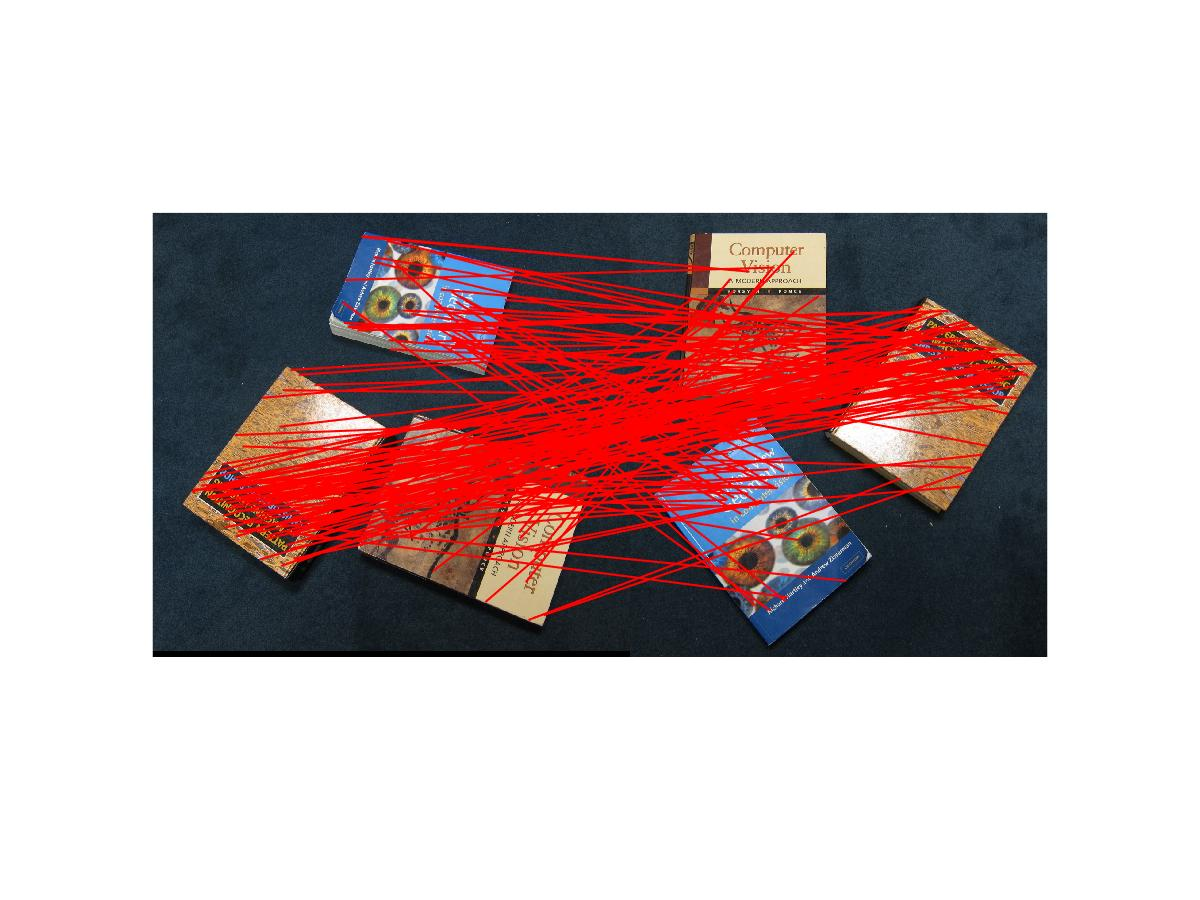
\includegraphics[width=0.42\linewidth]{../results/ImageMatchPFBook.jpg} & 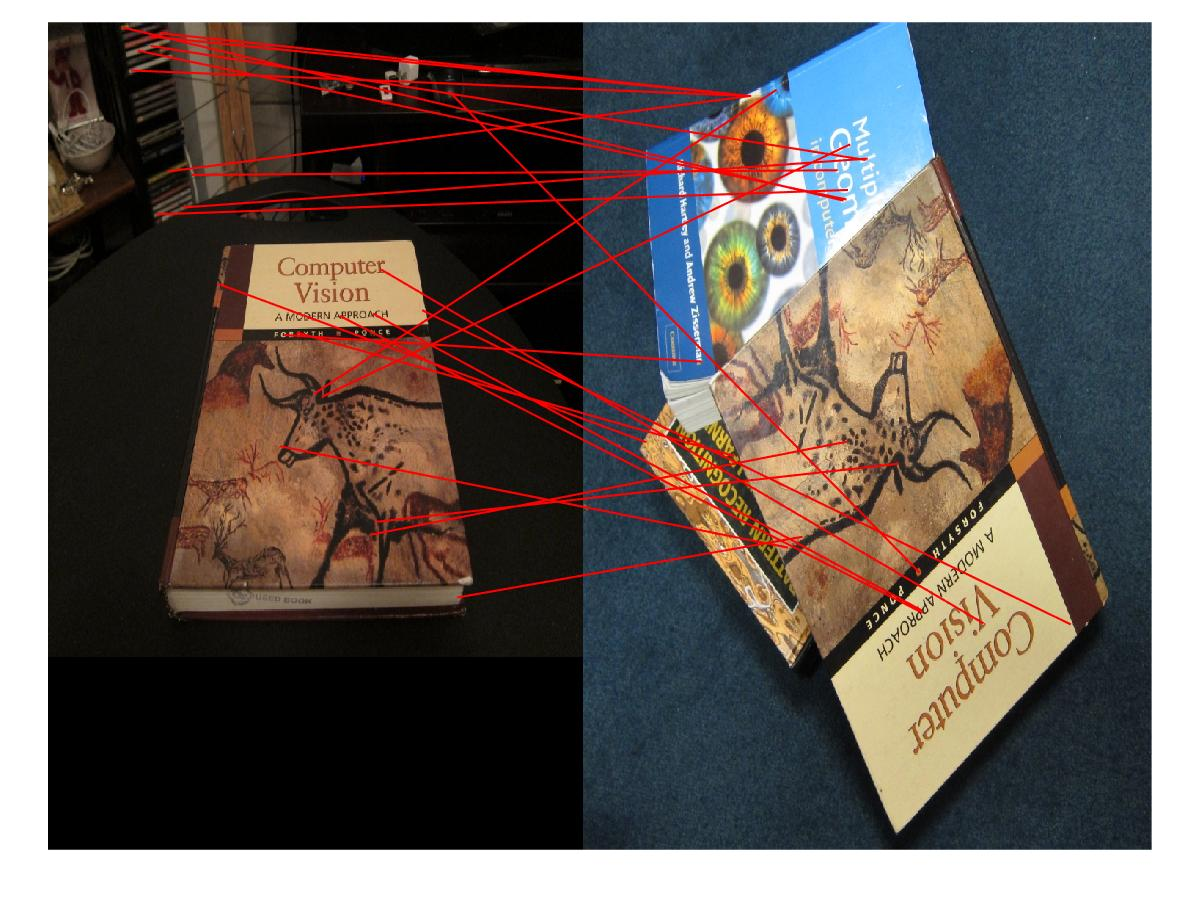
\includegraphics[width=0.42\linewidth]{../results/ImageMatchPFDeskPile.jpg} \\
  \hline
\end{tabular}
\caption{Output of \texttt{testMatches}}
\label{fig:testmatches}
\end{figure*}

\question{2.5}{briefRotTest}

Included in \texttt{code/briefRotTest.m} file. Results in figure (\ref{fig:rotationtest}).

\begin{figure*}[f]
\centering
  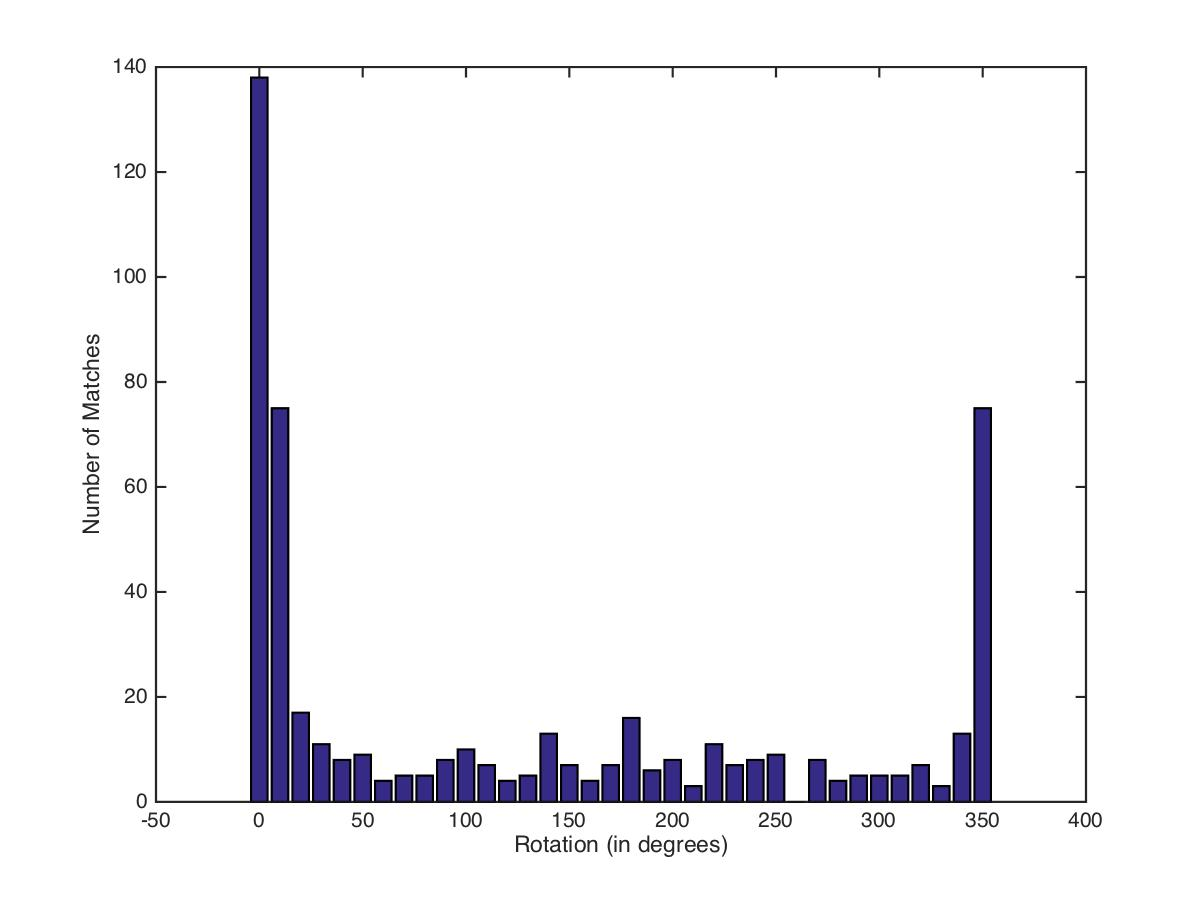
\includegraphics[width=0.9\linewidth]{../results/RotationError.jpg}
\caption{Output of \texttt{briefRotTest}}
\label{fig:rotationtest}
\end{figure*}

\question{3.1.a}{Equation for computing homography $H$}

Consider a single 3D point represented in two image capturing planes by two points $p = (x_1, y_1, 1)$ and $q = (x_2, y_2, 1)$ respectively. Our planar homography $H$ maps $p$ to $q$ through an affine operation.

$$\therefore q \equiv Hp$$

$$\therefore \lambda q = Hp$$

If $H=[a,b,c;d,e,f;g,h,i]$, then substituting $p = (x_1, y_1, 1)$ and $q = (x_2, y_2, 1)$ in $\lambda q = Hp$ gives:

$$\lambda = gx_1+hy_1+i$$
$$\lambda x_2 = ax_1+by_1+c$$
$$\lambda y_2 = dx_1+ey_1+f$$

Substituting $\lambda$ gives us the following two equations in the 9 unknows of matrix $H$:

$$(gx_1+hy_1+i) * x_2 = ax_1+by_1+c$$
$$(gx_1+hy_1+i) * y_2 = dx_1+ey_1+f$$

If we vectorize $H$ to $h=[a,b,c,d,e,f,g,h,i]'$, then $$A=[[x_1, y_1, 1, 0, 0, 0, -x_1x_2, -x_2y_1, -x_2]; [0,0,0,x_1,y_1,1,-x_1y_2,-y_1y_2 -y_2]]$$ The linear equations from further point correspondences can be stacked down as further rows in $A$ to obtain the final linear system $Ah=0$ to solve.

\question{3.1.b}{Elements in $H$}

We have seen that there are 9 unknown elements in $H=[a,b,c;d,e,f;g,h,i]$.

\question{3.1.c}{Required number of point correspondences to solve for $H$}

Even though there are 9 unknown elements in $H=[a,b,c;d,e,f;g,h,i]$, there are only 8 degrees of freedom because we need to know $H$ only up to a scaling factor $\lambda$. This is why we were able to resolve the three equations of $\lambda q = Hp$ to two by eliminating $\lambda$. Since each point correspondence gave us two equations and we have eight effective unknowns, we need \emph{four} point correspondences to determine $H$. 

\question{3.1.d}{Least squares solution for $H$}

Instead of solving for $Ah=0$ which may not have a solution due to the large number of constraint rows and noise in $A$, we instead solve for $h$ to minimize the $l_2$ nor of $Ah$.

$$\hat{h} = argmin_{||h||_2=1} \text{ } (||Ah||_2)^2 = argmin_{||h||_2=1} \text{ } ||h'A'Ah|| $$

Rayleigh Quotient for matrix $M$ and vector $x$ is given as 

$$R(M,x)=\frac{x'Mx}{x'x}$$

Also, $R(M,cx)=R(M,x)$ i.e. the vector $x$ that provides a particular value of Rayleigh Quotient for a given matrix $M$ is defined up to a scaling factor.

Rayleigh Quotient Theorem establishes that the vector $x$ that maximizes $R(M,x)$ is the eigenvector corresponding to the largest eigenvalue of $M$. Correspondingly, it also states that the vector $x$ that minimizes $R(M,x)$ is the eigenvector corresponding to the smallest eigenvalue of $M$. If $M=A'A$, then the vector $x$ that minimizes $R(A'A,x)$ is the smallest eigenvector of $A'A$ which we know is the smallest right singular vector of $A$. Hence, by calculating the \emph{SVD} of $A$, we can calculate $h$ that minimizes $||h'A'Ah||$. We do not have to worry about satisfying the norm condition $||h||_2=1$, because out of all minimizers of $R(A'A,x)$, SVD returns the smallest right singular vector which is normalized to already have a length of 1. Thus, we conveniently get a unique minimizer $h$ with a fixed scaling factor to 1.

\question{4.1}{computeH}

Included in \texttt{code/computeH.m} file.

\question{5.1}{imageStitching}

Included in \texttt{code/imageStitching.m} file. Result in figure (\ref{fig:noransacimagestitching}.a). Please zoom if result image is not clear.

\question{5.2}{imageStitching\_noClip}

Included in \texttt{code/imageStitching\_noClip.m} file. Result in figure (\ref{fig:noransacimagestitching}.b). Please zoom if result image is not clear.

\begin{figure*}[f]
\centering
\begin{tabular}{| c | c |}
  \hline
  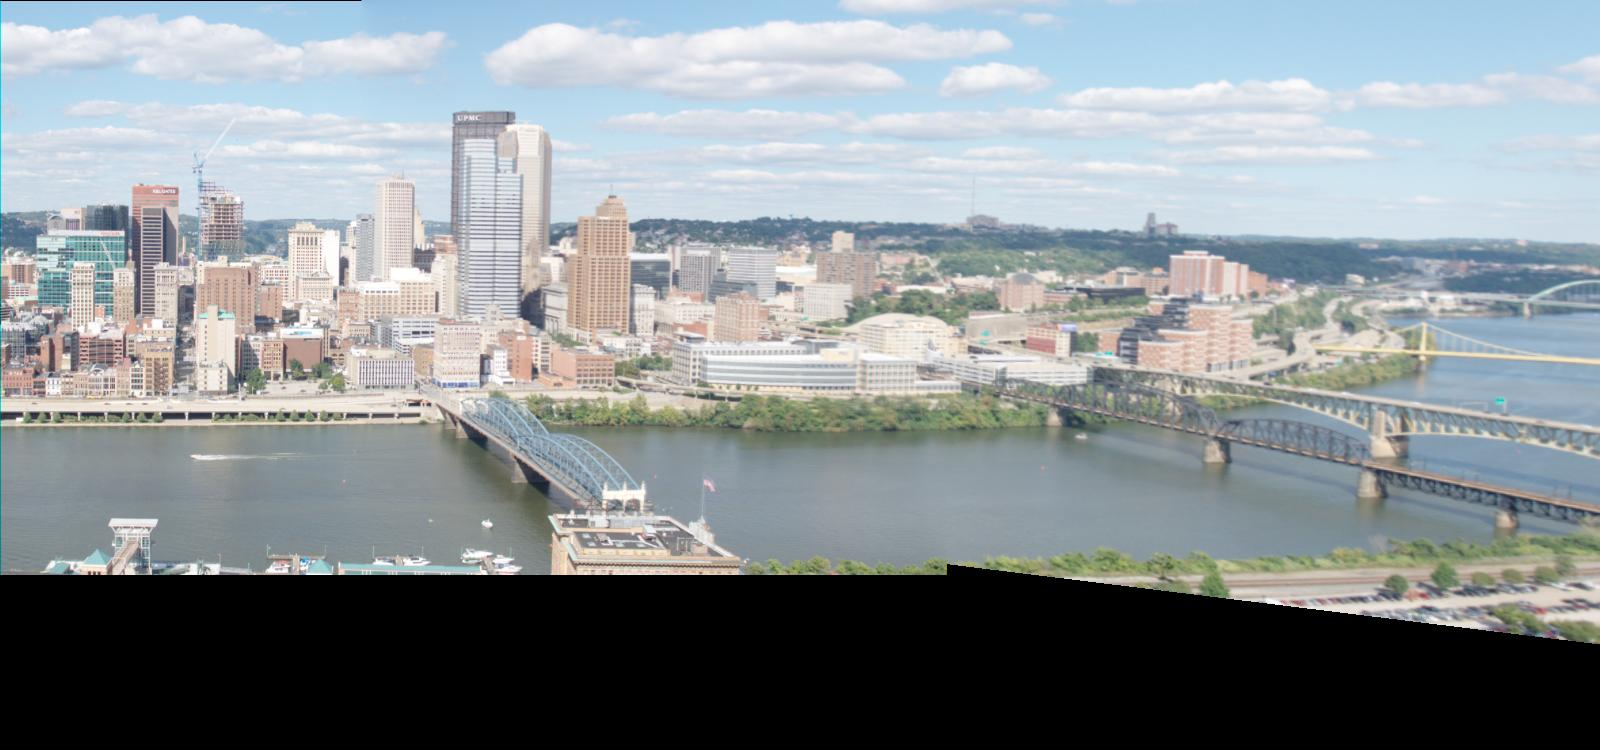
\includegraphics[width=0.42\linewidth]{../results/q5_1.jpg} & 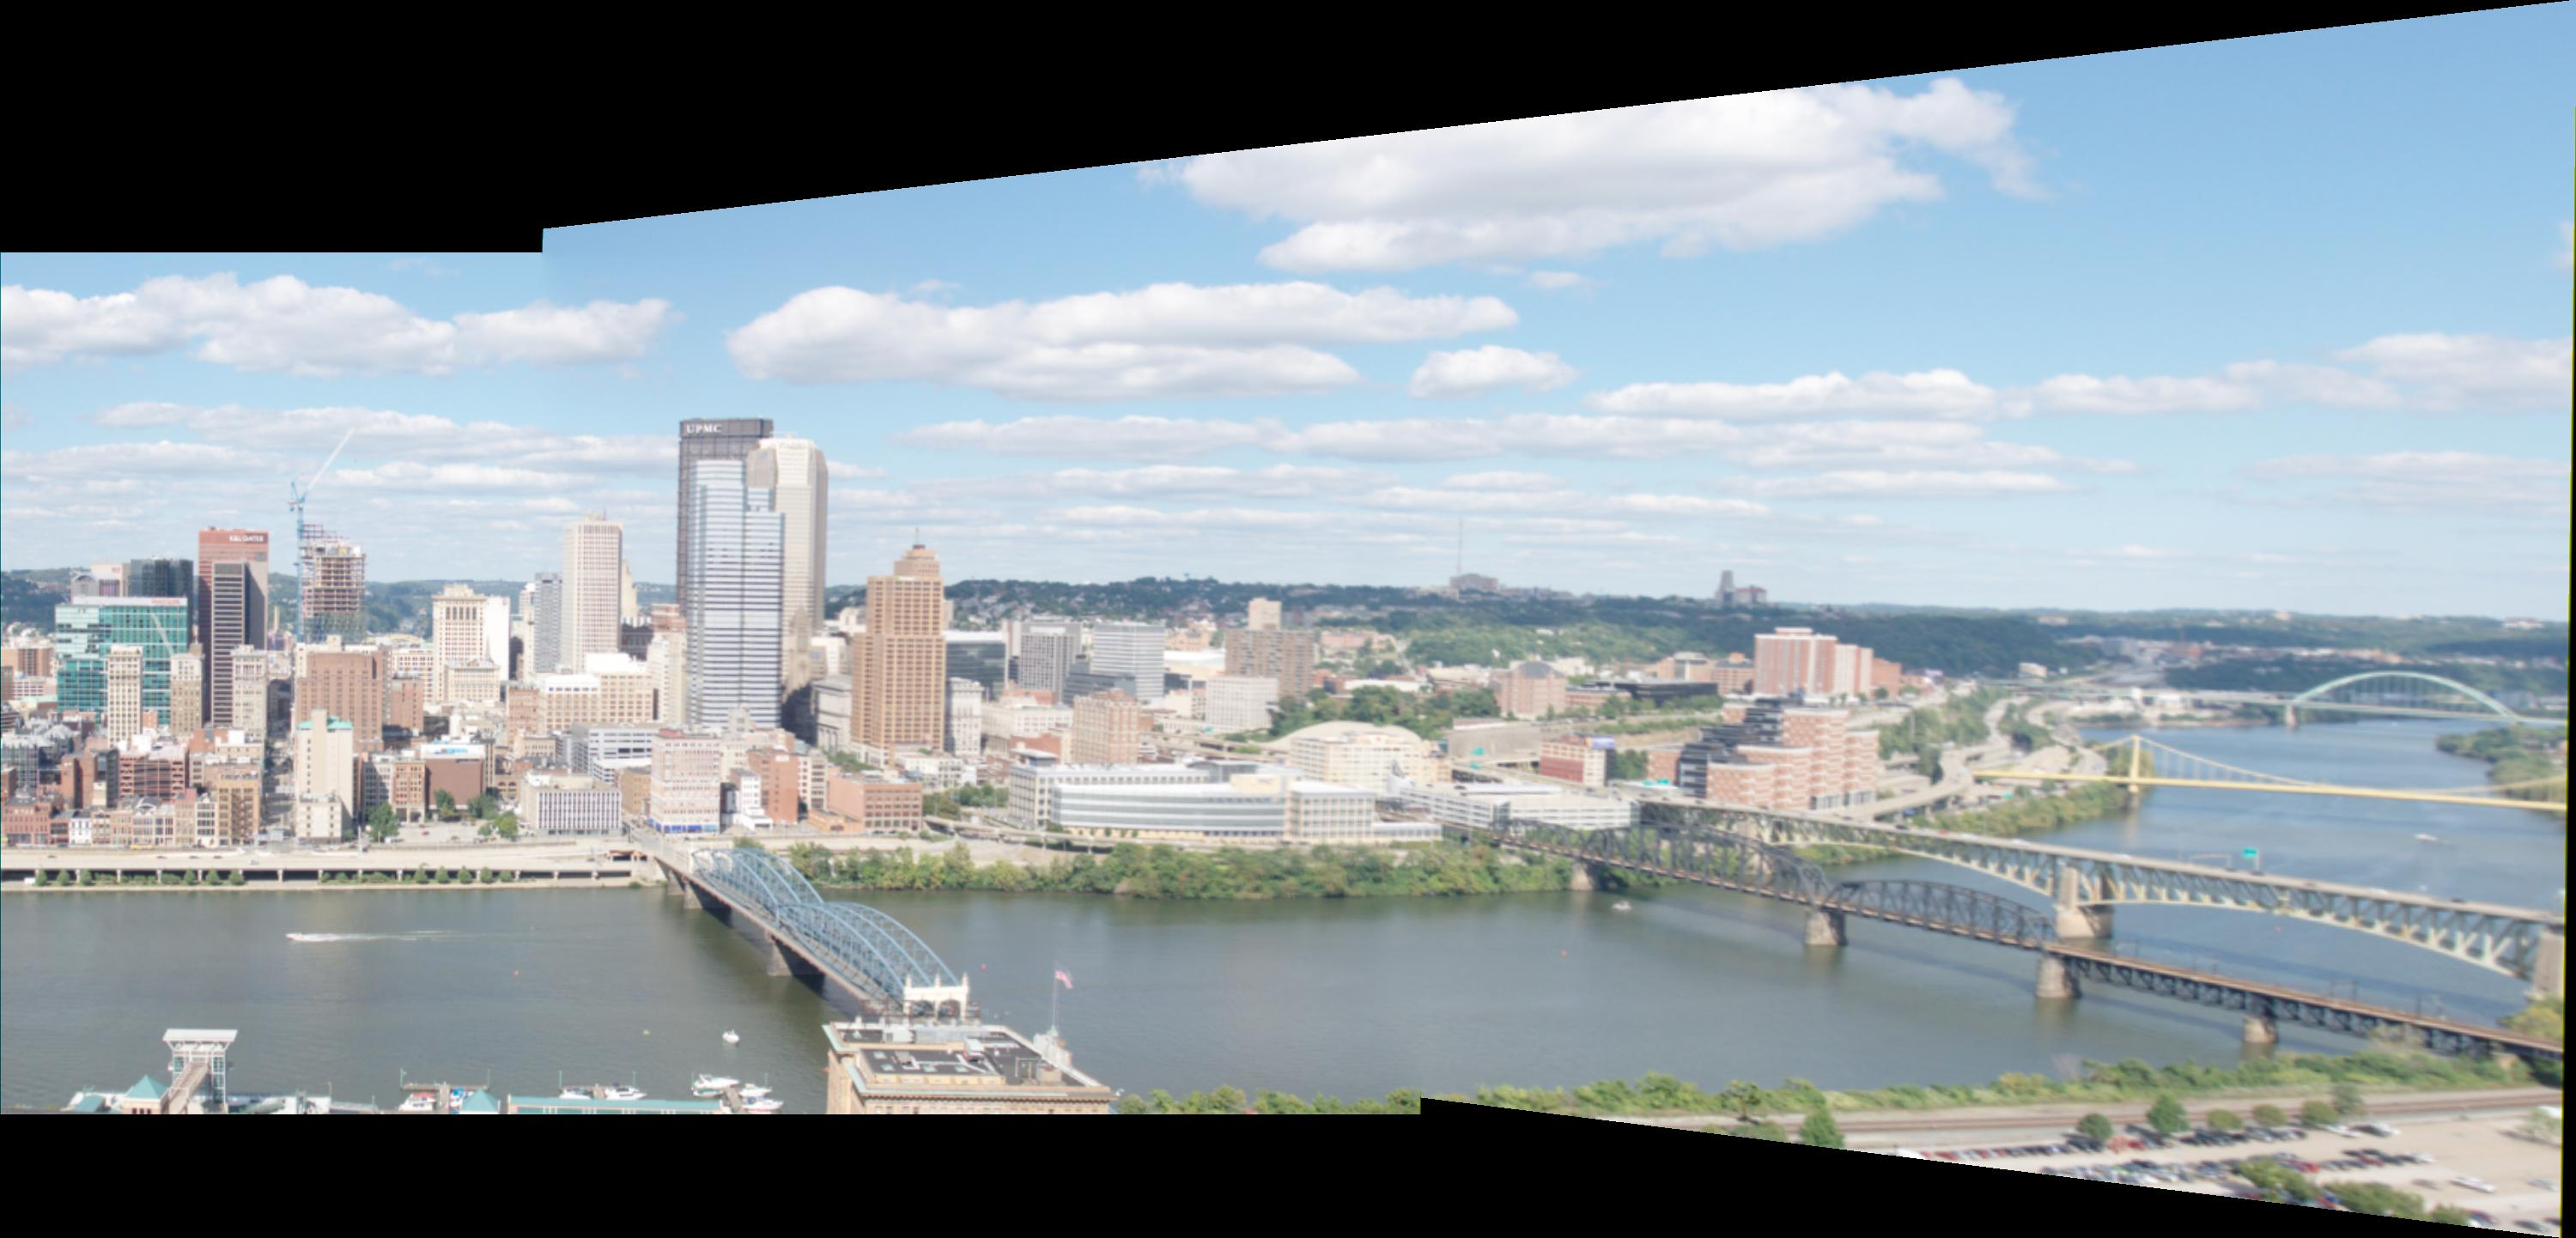
\includegraphics[width=0.42\linewidth]{../results/q5_2_pan.jpg} \\
  \hline
  (a) \texttt{imageStiching} output & (b) \texttt{imageStitching\_noClip} output \\
  \hline
\end{tabular}
\caption{Output of Image Stiching}
\label{fig:noransacimagestitching}
\end{figure*}

\question{6.1}{ransacH}

Included in \texttt{code/ransacH.m} file.

\question{6.2}{generatePanorama}

Included in \texttt{code/generatePanorama.m} file. Results in figure (\ref{fig:ransacimagestitching}). Please zoom if result image is not clear.

\begin{figure*}[f]
\centering
\begin{tabular}{| c | c |}
  \hline
  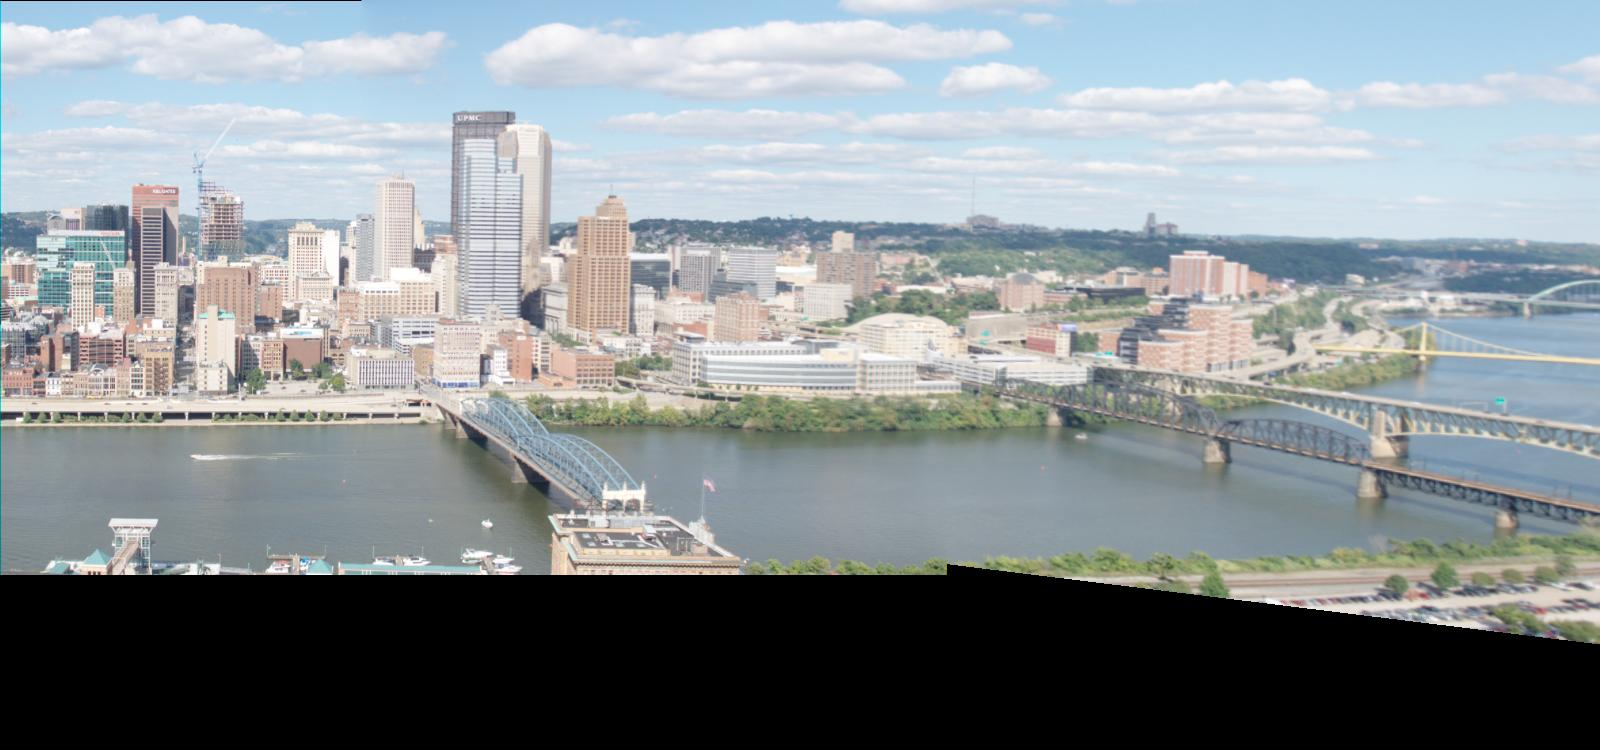
\includegraphics[width=0.42\linewidth]{../results/q6_1.jpg} & 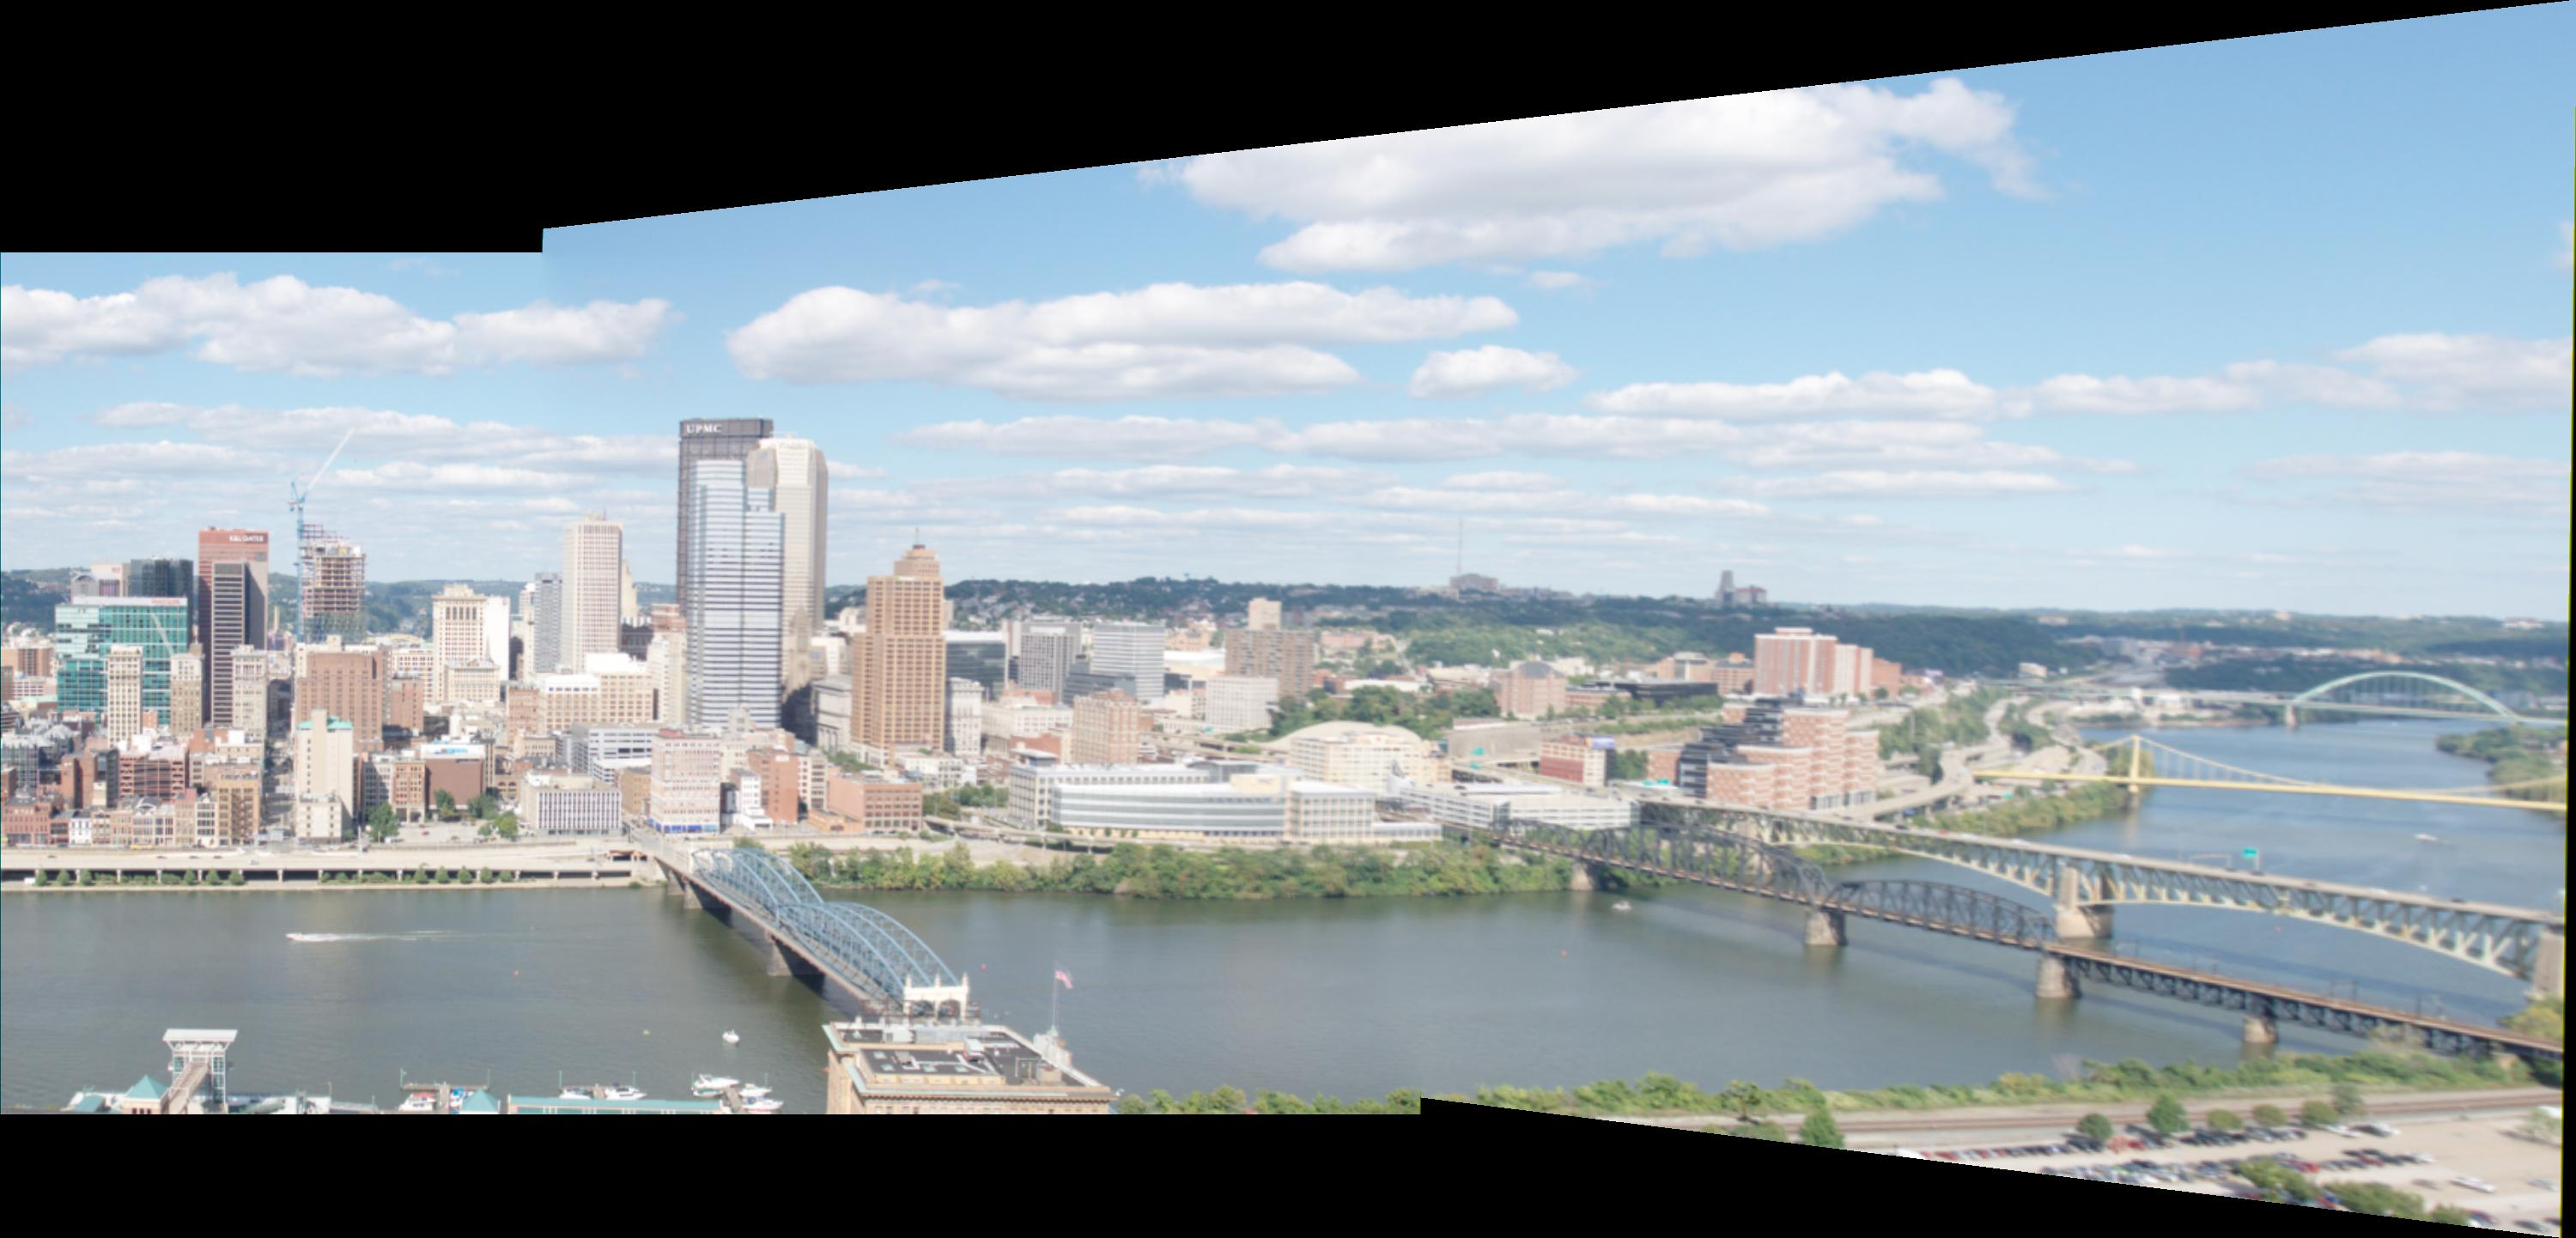
\includegraphics[width=0.42\linewidth]{../results/q6_2_pan.jpg} \\
  \hline
  (a) \texttt{imageStiching} output & (b) \texttt{imageStitching\_noClip} output \\
  \hline
\end{tabular}
\caption{Output of RANSAC Image Stiching}
\label{fig:ransacimagestitching}
\end{figure*}

\question{7.1}{ec\_1}

Included in \texttt{code/ec\_1.m} file. Results in figure (\ref{fig:briefrotationenhancement}). We decided to enhance the \texttt{computeBrief} function so as to include BRIEF descriptors on the rotated versions of the input image. We chose all rotations of the image spaced 30 degrees apart i.e. $30, 60, .., 360$. Figure (\ref{fig:briefrotationenhancement}.a) shows the number of matches without BRIEF enhancement while figure (\ref{fig:briefrotationenhancement}.b) shows the number of matches with the suggested BRIEF enhancement. We observe that the number of matches has significantly improved between the original image and its rotated version where rotation is on the X-axis of the figure, while keeping the number of matches between the original image and its unrotated version (at 360 degrees in the figure) fairly high.

\begin{figure*}[f]
\centering
\begin{tabular}{| c | c |}
  \hline
  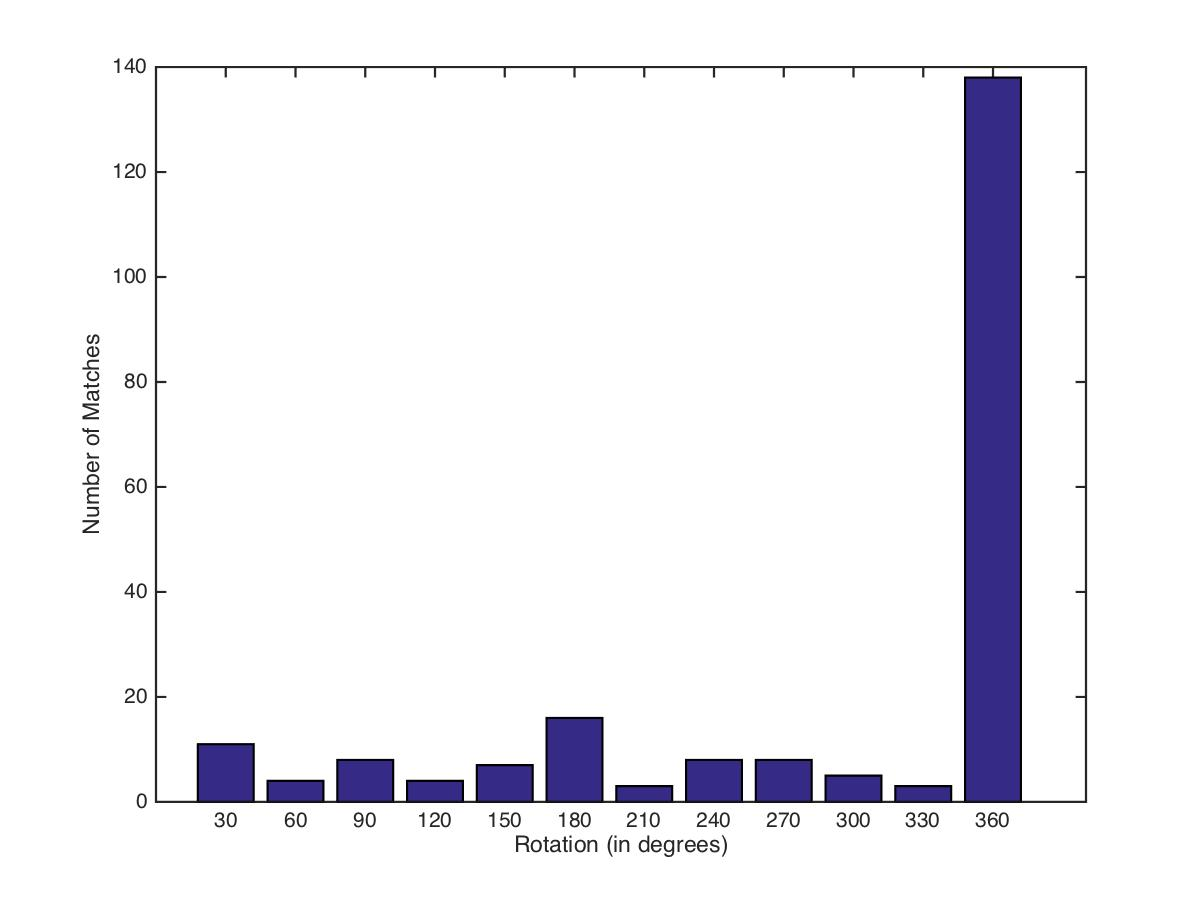
\includegraphics[width=0.42\linewidth]{../results/EC1_RotationError_1.jpg} & 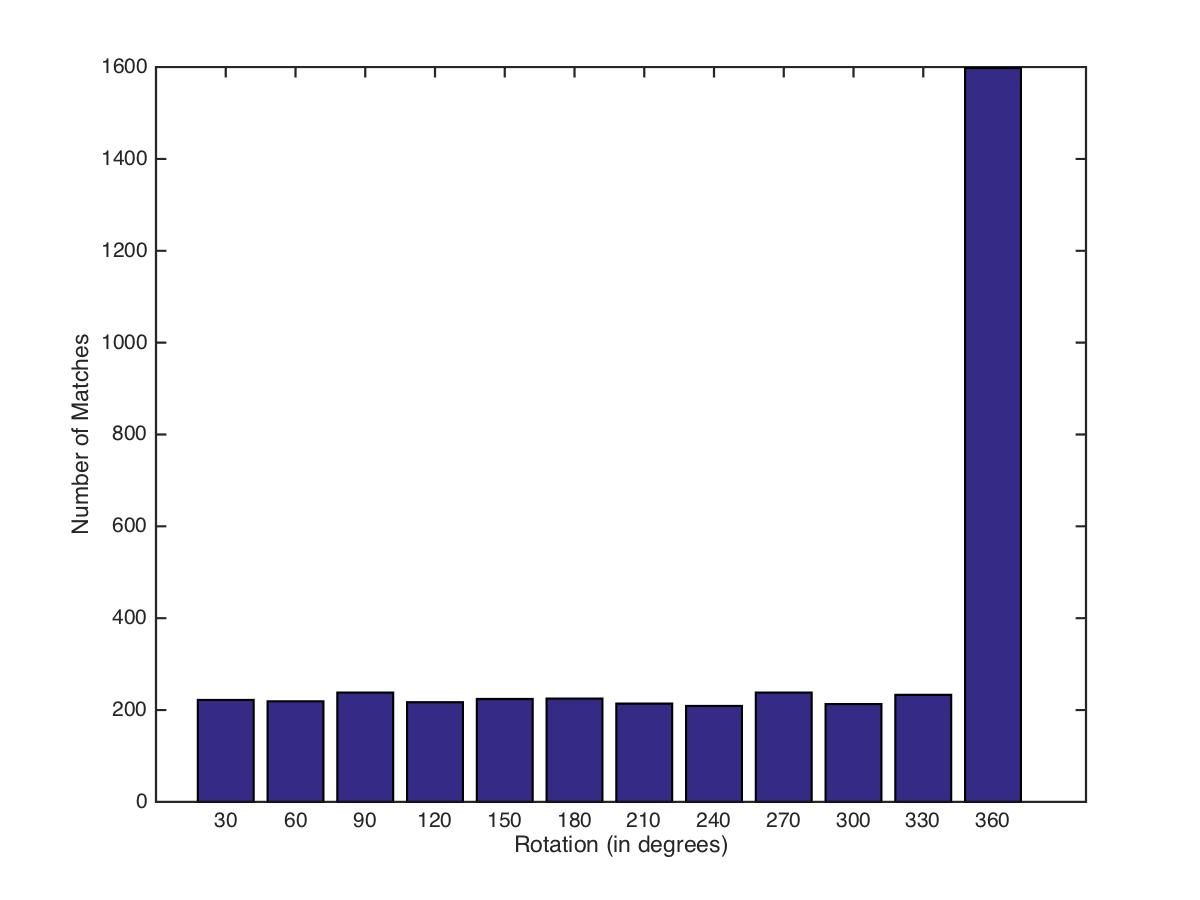
\includegraphics[width=0.42\linewidth]{../results/EC1_RotationError_2.jpg} \\
  \hline
  (a) Matches w/o BRIEF Enhancement & (b) Matches with BRIEF Enhancement \\
  \hline
\end{tabular}
\caption{Output of BRIEF Descriptor Enhancement for Rotation}
\label{fig:briefrotationenhancement}
\end{figure*}

\question{7.2}{ec\_2}

Included in \texttt{code/ec\_2.m} file. Results in figure (\ref{fig:briefscalingenhancement}). We decided to enhance the \texttt{computeBrief} function so as to include BRIEF descriptors on the scaled versions of the input image. We chose the following scalings of the original image for enhancement $0.4, 0.7, 1.0$. Figure (\ref{fig:briefscalingenhancement}.a) shows the number of matches without BRIEF enhancement while figure (\ref{fig:briefscalingenhancement}.b) shows the number of matches with the suggested BRIEF enhancement. We observe that the number of matches has significantly improved between the original image and its scaled version where the applied scaling for the matched image is on the X-axis of the figure, while keeping the number of matches between the original image and its unscaled version (at 1.0 scaling in the figure) fairly high. It is odd that the absolute number of matches between the original image and its unscaled version is lower in the case of the BRIEF descriptor enhancement than in the case without the enhancement. This is not the case in the case of BRIEF enhancement to handle image rotations.

\begin{figure*}[f]
\centering
\begin{tabular}{| c | c |}
  \hline
  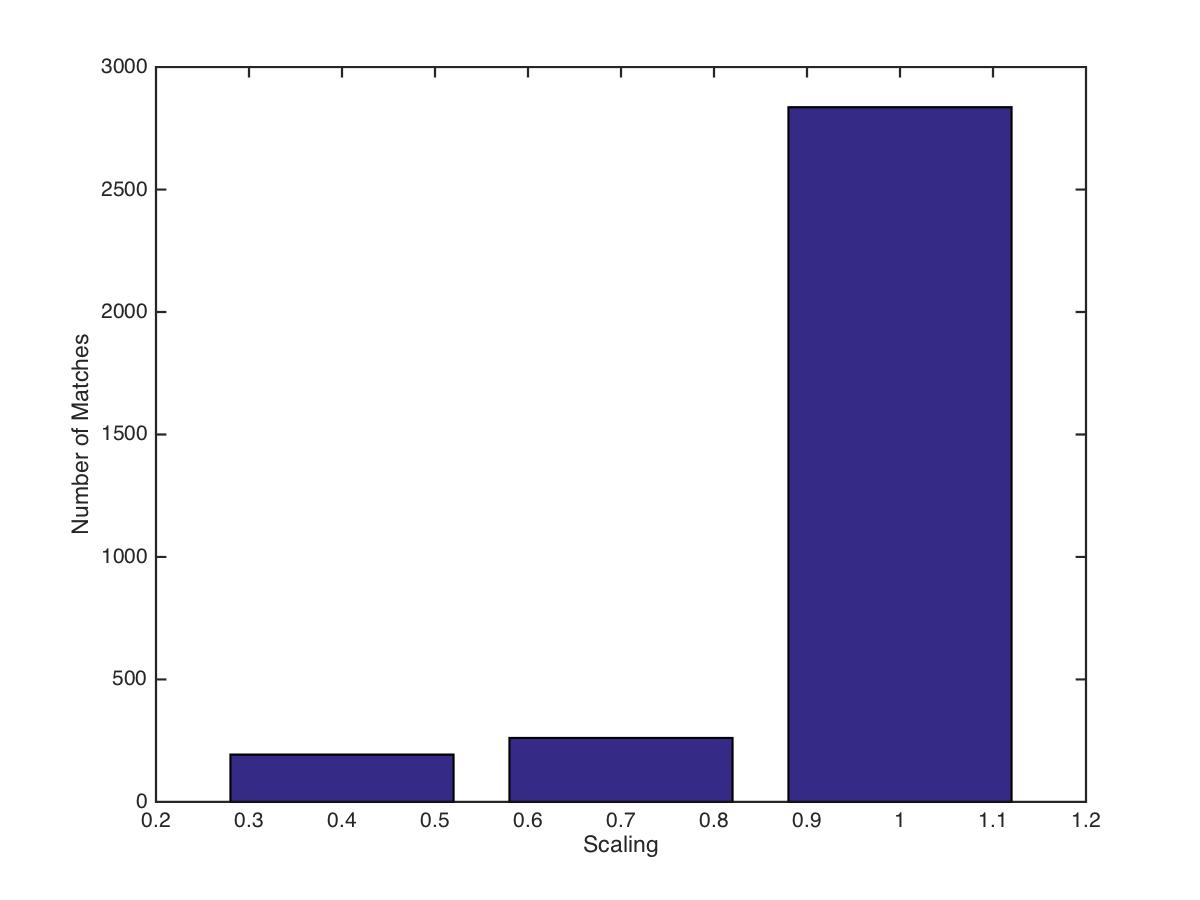
\includegraphics[width=0.42\linewidth]{../results/EC2_ScalingError_1.jpg} & 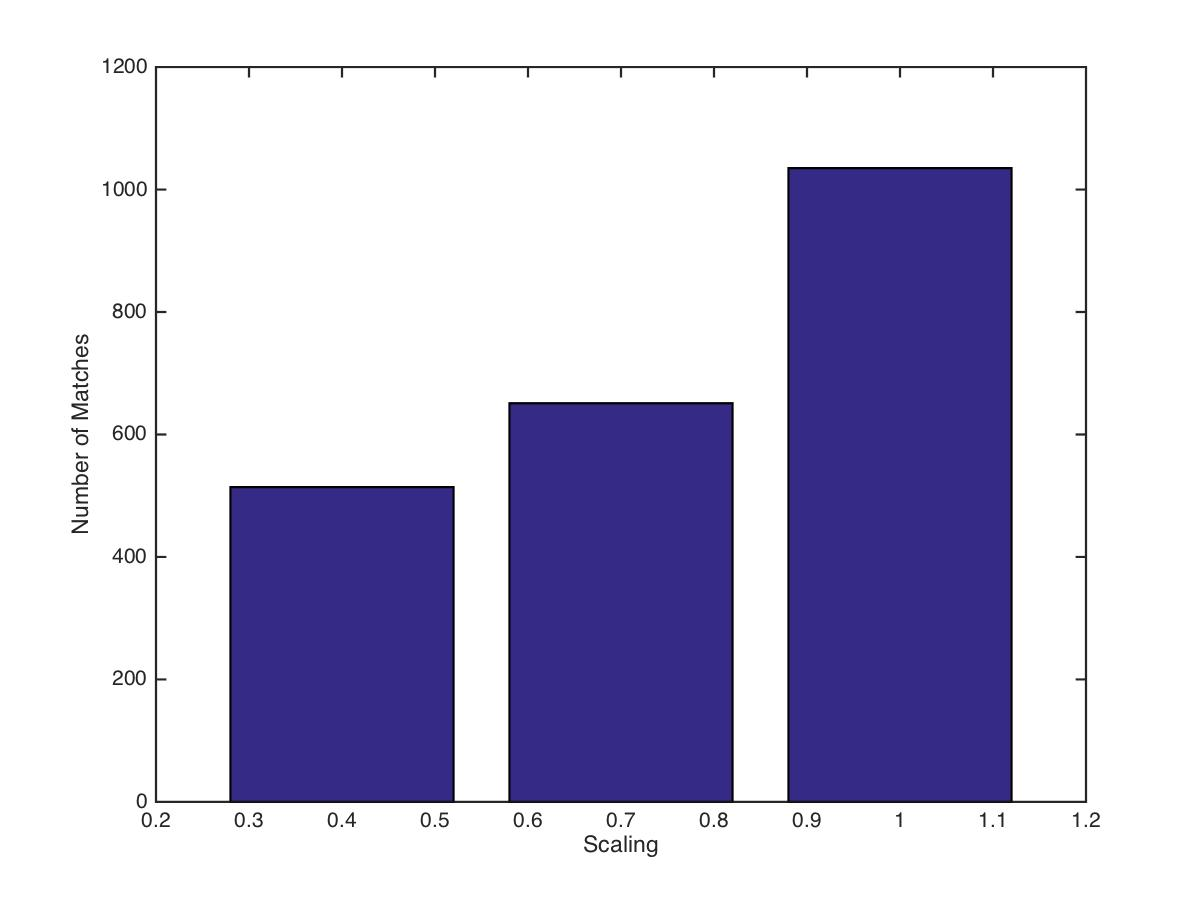
\includegraphics[width=0.42\linewidth]{../results/EC2_ScalingError_2.jpg} \\
  \hline
  (a) Matches w/o BRIEF Enhancement & (b) Matches with BRIEF Enhancement \\
  \hline
\end{tabular}
\caption{Output of BRIEF Descriptor Enhancement for Scaling}
\label{fig:briefscalingenhancement}
\end{figure*}

\end{document}

